
\begin{figure}
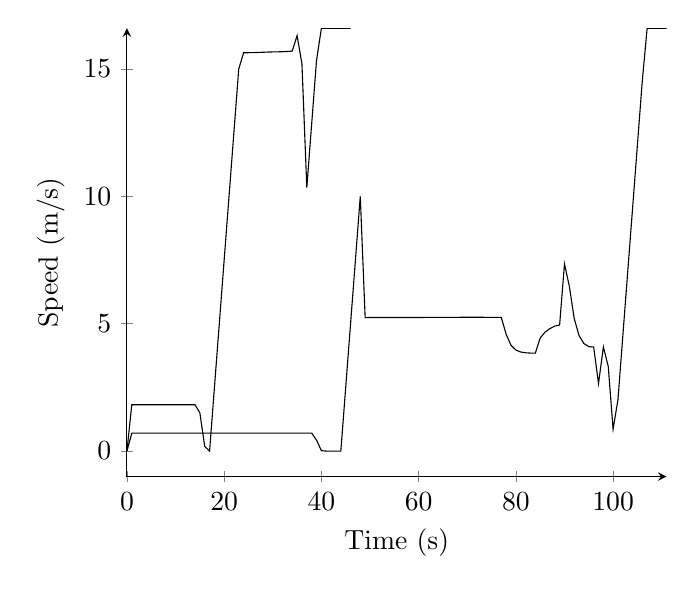
\begin{tikzpicture}
\begin{axis}[
legend style={anchor=west},
axis x line=bottom,
axis y line=left,
ymin=-1,
xlabel=Time (s),
ylabel=Speed (m/s),
]
\addplot[] coordinates {
(0, 0.0)
(1, 0.703243082183)
(2, 0.703244234986)
(3, 0.703245454833)
(4, 0.70324674707)
(5, 0.703248117593)
(6, 0.703249572915)
(7, 0.703251120248)
(8, 0.703252767597)
(9, 0.703254523863)
(10, 0.703256398977)
(11, 0.703258404037)
(12, 0.703260551487)
(13, 0.703262855316)
(14, 0.703122467028)
(15, 0.703124826049)
(16, 0.703127371112)
(17, 0.70313012264)
(18, 0.703133103982)
(19, 0.703174493278)
(20, 0.703178470484)
(21, 0.70318281251)
(22, 0.703187566428)
(23, 0.703192787347)
(24, 0.703198540167)
(25, 0.703204901802)
(26, 0.703211964042)
(27, 0.703219837259)
(28, 0.703228655283)
(29, 0.703238581897)
(30, 0.703249819619)
(31, 0.703262621784)
(32, 0.703277309485)
(33, 0.703294295861)
(34, 0.703314121814)
(35, 0.70333751013)
(36, 0.70336545041)
(37, 0.703399338178)
(38, 0.703441214935)
(39, 0.431417870457)
(40, 0.0154901195954)
(41, 0.0)
(42, 0.0)
(43, 0.0)
(44, 0.0)
(45, 2.5)
(46, 5.0)
(47, 7.5)
(48, 10.0)
(49, 5.24155845104)
(50, 5.24179875953)
(51, 5.24205445947)
(52, 5.24232689465)
(53, 5.24261755884)
(54, 5.2429281164)
(55, 5.24326042621)
(56, 5.24361656959)
(57, 5.24399888307)
(58, 5.24440999692)
(59, 5.24485288063)
(60, 5.24533089686)
(61, 5.24584786563)
(62, 5.24640814118)
(63, 5.24701670422)
(64, 5.24767927348)
(65, 5.24840244105)
(66, 5.24919383773)
(67, 5.250062336)
(68, 5.25101830107)
(69, 5.25207390312)
(70, 5.2530742012)
(71, 5.25334473566)
(72, 5.25364676425)
(73, 5.25398538166)
(74, 5.24793913146)
(75, 5.24808359733)
(76, 5.24824799281)
(77, 5.2484361699)
(78, 4.58608523363)
(79, 4.15344772617)
(80, 3.96565918907)
(81, 3.88903619103)
(82, 3.85875574788)
(83, 3.84708002761)
(84, 3.842781287)
(85, 4.43604725574)
(86, 4.66920833911)
(87, 4.80888027009)
(88, 4.9061489458)
(89, 4.94945232146)
(90, 7.34708274401)
(91, 6.46974690168)
(92, 5.20556660685)
(93, 4.53041747933)
(94, 4.22043453269)
(95, 4.10028714801)
(96, 4.08657623381)
(97, 2.65301516026)
(98, 4.08543556531)
(99, 3.32827354257)
(100, 0.86129760134)
(101, 2.0164425018)
(102, 4.5164425018)
(103, 7.0164425018)
(104, 9.5164425018)
(105, 12.0164425018)
(106, 14.5164425018)
(107, 16.6)
(108, 16.6)
(109, 16.6)
(110, 16.6)
(111, 16.6)
};
\addplot[] coordinates {
(0, 0.0)
(1, 1.8200928686)
(2, 1.82010110249)
(3, 1.8201106908)
(4, 1.82012195145)
(5, 1.82013530279)
(6, 1.81978230215)
(7, 1.81979948384)
(8, 1.81991994917)
(9, 1.81994981207)
(10, 1.81998794532)
(11, 1.82003783861)
(12, 1.82010513697)
(13, 1.82019957369)
(14, 1.82033946403)
(15, 1.50145312164)
(16, 0.18501103285)
(17, 0.0)
(18, 2.5)
(19, 5.0)
(20, 7.5)
(21, 10.0)
(22, 12.5)
(23, 15.0)
(24, 15.6363617772)
(25, 15.6396679699)
(26, 15.6437881552)
(27, 15.6490135793)
(28, 15.655778634)
(29, 15.6647545585)
(30, 15.6693111948)
(31, 15.6729311046)
(32, 15.6783113601)
(33, 15.686817291)
(34, 15.7014621188)
(35, 16.3106933916)
(36, 15.2001777225)
(37, 10.3415238823)
(38, 12.8415238823)
(39, 15.3415238823)
(40, 16.6)
(41, 16.6)
(42, 16.6)
(43, 16.6)
(44, 16.6)
(45, 16.6)
(46, 16.6)
};

\end{axis}
\end{tikzpicture}
\label{tik:100:6_O, 6_O.-30, 5_N, 4_N, 4_N.-60, 3_O}
\caption{100 percent diving with GSC on route $6_O, 6_O.-30, 5_N, 4_N, 4_N.-60, 3_O$}
\end{figure}
